% !TeX spellcheck = en_US
\documentclass[usenames,dvipsnames]{beamer}
\setbeamertemplate{navigation symbols}{}

\usepackage{mathtools, cases, graphicx, xcolor, graphics, mathrsfs, dsfont, amssymb, multirow, dcolumn, natbib, hyperref, multicol, subcaption, changepage, booktabs, caption, appendixnumberbeamer, enumerate}
\usepackage{lmodern} % http://ctan.org/pkg/lm
\usepackage{tikz}
\usepackage{dcolumn}
\usepackage{tabularx}

\usetikzlibrary{matrix,shapes,arrows,fit,tikzmark}
\newcolumntype{.}{D{.}{.}{-1}}

% Some options common to all the nodes and paths
\tikzset{   
	every picture/.style={remember picture,baseline},
	every node/.style={anchor=base,align=center,outer sep=1.5pt},
	every path/.style={thick},
}

\newcommand\marktopleft[1]{%
	\tikz[overlay,remember picture] 
	\node (marker-#1-a) at (.1em,.3em) {};%
}

\newcommand\markbottomrightred[1]{%
	\tikz[overlay,remember picture] 
	\node (marker-#1-b) at (.1em,.3em) {};%
	\tikz[overlay,remember picture,inner sep=3pt]
	\node[draw=Red,rounded corners,fit=(marker-#1-a.north west) (marker-#1-b.south east)] {};%
}

\newcommand\markbottomrightblue[1]{%
	\tikz[overlay,remember picture] 
	\node (marker-#1-b) at (.1em,.3em) {};%
	\tikz[overlay,remember picture,inner sep=3pt]
	\node[draw=Blue,rounded corners,fit=(marker-#1-a.north west) (marker-#1-b.south east)] {};%
}
\newcommand\markbottomrightgreen[1]{%
	\tikz[overlay,remember picture] 
	\node (marker-#1-b) at (.1em,.3em) {};%
	\tikz[overlay,remember picture,inner sep=3pt]
	\node[draw=Green, rounded corners,fit=(marker-#1-a.north west) (marker-#1-b.south east)] {};%
}

\usepackage[flushleft]{threeparttable}
\usepackage[utf8]{inputenc}
\usepackage[T1]{fontenc}
%\usetheme{Warsaw}
\usetheme{Boadilla}

%\newcommand*\oldmacro{}%
%\let\oldmacro\insertshorttitle%
%\renewcommand*\insertshorttitle{%
%	\oldmacro\hfill%
%	\insertframenumber\,/\,\inserttotalframenumber}
%\setcounter{tocdepth}{1}

\begin{document}
	
	\title[Inter-generational conflict and labor share]{Inter-generational conflict and the declining labor share}
	\author[Fabien Petit]{Fabien Petit\inst{1}}
	\institute[AMSE]{\inst{1} Aix-Marseille University, CNRS, EHESS, Centrale Marseille, AMSE}
	\date{March 27, 2020}
	
	\begin{frame}
		\titlepage
		\vspace{-0.5cm}
		\begin{figure}
			\begin{subfigure}[h]{0.49\linewidth}
				\centering
				
\includegraphics[width=0.7\linewidth]{Pictures/amu} 
			\end{subfigure}
			%%%
			\begin{subfigure}[h]{0.49\linewidth}
				\centering
				
\includegraphics[width=0.7\linewidth]{Pictures/amse.png}
			\end{subfigure}
		\end{figure}
	\end{frame}
	\section{Introduction}
	\begin{frame}\frametitle{Since World War II} % What's the research question ?
		\begin{enumerate}\setbeamertemplate{enumerate items}[default]
			\item Appearance of the \textbf{baby-boomers' cohort} in many OECD countries
			\vspace{2em}
			\item \textbf{Declining labor income share} since the entry of the boomers on the labor market
			\begin{itemize}
				\item Biased technical change, institutions, globalization ?
			\end{itemize}
		\end{enumerate}
		\vfill
		\begin{itemize}
			\item[] {\Large \textit{How does age structure affect the income allocation\\\vspace{1em}
					between capital and labor in high-income countries ?}}
		\end{itemize}
	\end{frame}
	\begin{frame}\frametitle{Why would this matter ?}
		\begin{itemize}
			\item[$\Rightarrow$] Aging population in many OECD countries
		\end{itemize}
		\begin{figure}[b]
			< Old-age dependency ratio figure >
		\end{figure}
	\end{frame}
	\begin{frame}\frametitle{What do we know ?}
		\begin{itemize}
			\item Population aging affects the labor share \textbf{through capital accumulation}
			\begin{itemize}
				\item {\scriptsize\color{CadetBlue}\textbf{\cite{Schmidt2013}}}
			\end{itemize}
			\vspace{2em}
			\item \textbf{Biased technical change} is the long-run response of firms to thwart \textbf{workers empowerment}
			\begin{itemize}
				\item {\scriptsize\color{CadetBlue}\textbf{\cite{Caballero1998}}; \cite{Blanchard1997}; \cite{Bentolila2003}; \cite{Acemoglu2002}; \cite{Karabarbounis2014}}
			\end{itemize}
			\vspace{2em}
			\item \textbf{Inter-generational conflict} over the public budget allocation
				\begin{itemize}
					\item {\scriptsize\color{CadetBlue}\textbf{\cite{Gonzalez-Eiras2012}}; \cite{Lancia2012}; \cite{Busemeyer2009}; \cite{Sorensen2013}; \cite{Jager2016}}
				\end{itemize}
		\end{itemize}
	\end{frame}
	\begin{frame}\frametitle{What I do ?}
		\begin{enumerate}\setbeamertemplate{enumerate items}[default]
			\item OLG model focusing on two elements:
			\begin{itemize}
				\item \textbf{Direct cohort effect}: factor accumulation
				\item \textbf{Indirect policy mechanism}: age-structure determines labor market institutions
			\end{itemize}
			\vspace{2em}
			\item \textbf{Calibration} to analyze the co-movement between labor share and age-structure
			\begin{itemize}
				\item France and the United-States
			\end{itemize}
			\vspace{2em}
			\item \textbf{Quantify} the role of population growth and survival rate
			%			\item Important implications for predicted labor share
		\end{enumerate}
	\end{frame}
	\begin{frame} \frametitle{Outline}
		\tableofcontents[sectionstyle=show, hideallsubsections]
	\end{frame}

\AtBeginSection[]
{
	\begin{frame}<beamer>
		\frametitle{Outline}
		\tableofcontents[currentsection]
	\end{frame}
}

	\section{Theoretical Framework}
	\begin{frame}[label = olgmodel]\frametitle{Overlapping generations model}
		\begin{itemize}
			\item \textbf{Standard 2-period OLG model} with logarithmic utility function and CES production function %\hyperlink{preferences<1>}{\beamergotobutton{Details}}
			\begin{itemize}
				\item Closed economy and capital fully depreciates between two periods
				\item Perfect annuities market
			\end{itemize}
		\vspace{1em}
			\item Each cohort: continuum of homogeneous agents
			\begin{itemize}
				\item Young households: supply labor inelastically, earn income, pay taxes, consume and save for retirement
				\item Old households: consume the return on their savings, pay taxes and derive utility from government health spending
			\end{itemize}
		\end{itemize}
	\end{frame}
	\begin{frame}\frametitle{Diagram of the model}
		\begin{figure}[ht]
			\centering
			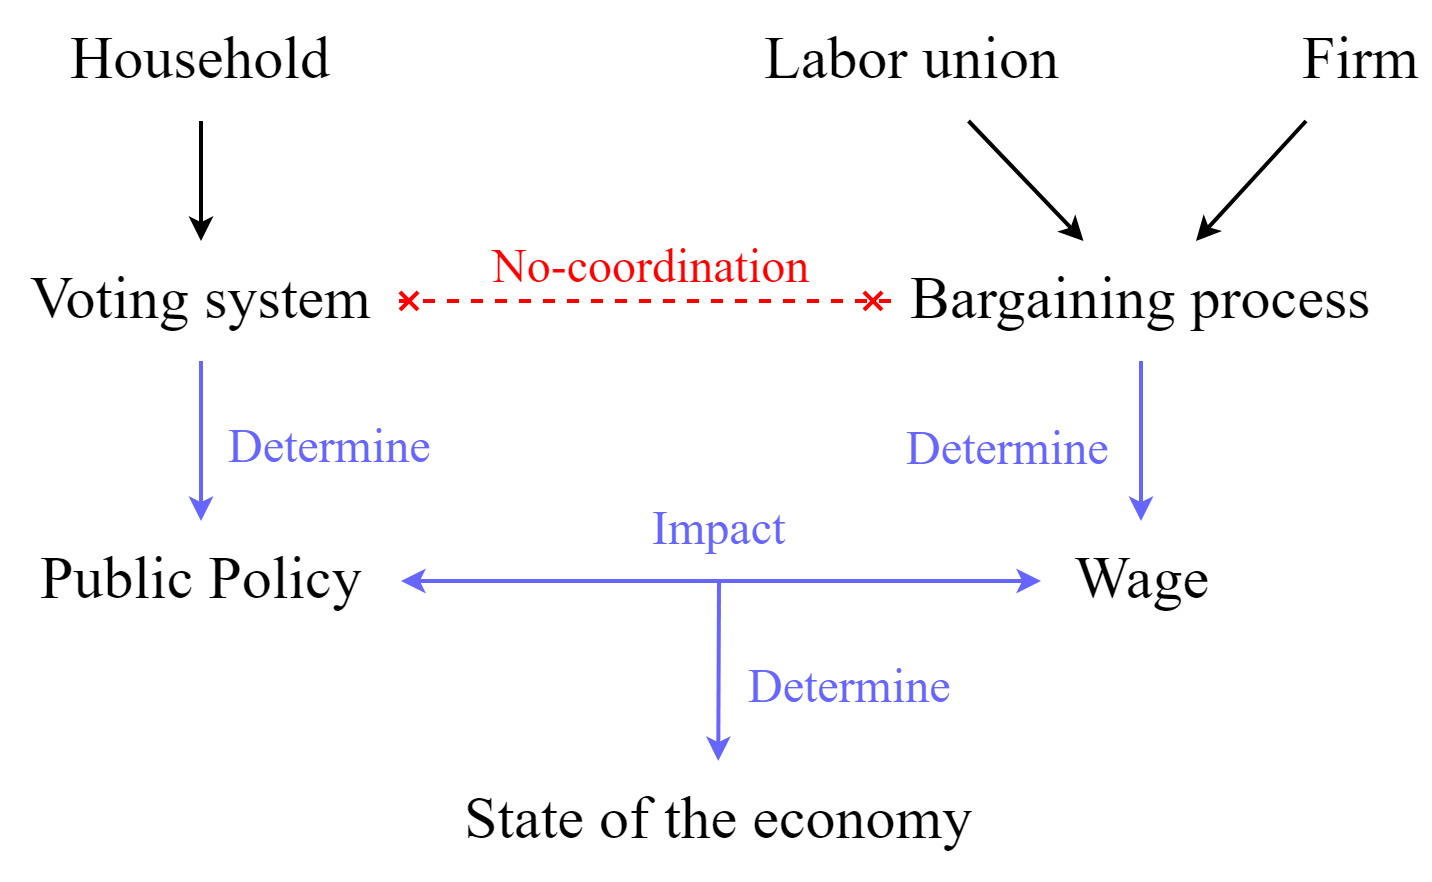
\includegraphics[width=\linewidth]{Diagrams/model_diagram.png}
		\end{figure}
	\end{frame}
	\begin{frame}\frametitle{Public policy preferences}
		\begin{itemize}
			\item \textbf{Age-related conflict} in the public policy:
			\begin{itemize}
				\item Young households desire more unemployment benefit ($b$)
				\item Old households desire more health spending ($h$)
				\item Both desire less taxes ($\tau$)
			\end{itemize}
			\vspace{1em}
			\item Solved with \textbf{probabilistic voting}: public policy depends on...
			\begin{enumerate}\setbeamertemplate{enumerate items}[default]
				\item Macroeconomic variables (\textit{wage rate, unemployment rate, etc.})
				\item Preference for government health spending
				\item Weight of the young generation within the social welfare function ($\textcolor{red}{\eta_t}$)
			\end{enumerate}
			\vspace{1em}
			\[
			\textcolor{red}{\eta_t} = \frac{n_t}{p_t}\frac{1+\alpha p_{t+1}}{\omega}\  \hspace{3em}
			\begin{array}{l}
			n~~\text{population growth}\\p~~\text{survival rate}\\\alpha~~\text{discount rate}\\\omega~~\text{relative per-capita influence}\\~~~~\text{of old households}
			\end{array}
			\]
		\end{itemize}
	\end{frame}
	\begin{frame}
		\begin{itemize}
			\item Maximization program characterizing equilibrium policy choices in period $t$ :
		\end{itemize}
		\begin{align*}
		\max_{\lbrace\tau_t, b_t, h_t\rbrace\geq 0} &\ln(1-\tau_t) +\beta \ln h_t + \textcolor{red}{\eta_t} \ln\left[(1-u_t)(1-\tau_t)w_t + u_t b_t\right] + \dots\\
		\text{s.t.} ~~ &\tau_t Y_t = b_t u_t N_t^y + h_t N_t^o
		\end{align*}
		$\textcolor{red}{\eta_t}$ the weight of the young generation within the social welfare function :\\
		\begin{equation*}
		\textcolor{red}{\eta_t} = \frac{n_t}{p_t}\frac{1+\alpha p_{t+1}}{\omega}
		\end{equation*}
	\end{frame}
	\begin{frame}
		\begin{itemize}
			\item Focusing on the interior solution, first order conditions give :
			\begin{align*}
			\frac{b_t}{(1-\tau_t)w_t} &= \frac{1-u_t}{u_t} \left(\textcolor{red}{\eta_t}\frac{1-\theta_t}{\theta_t}- 1\right)\\
			\tau_t &= 1 - \left[\left(1-\theta_t\right)\left(1+\beta+\textcolor{red}{\eta_t}\right)\right]^{-1}\\
			h_t &= \left(\tau_t \frac{Y_t}{N_t^y} - b_t u_t\right)\frac{n_t}{p_t}
			\end{align*}
		\end{itemize}
	\end{frame}	
	\begin{frame}\frametitle{Wage bargaining}
		\begin{itemize}
			\item Right-to-manage model \textit{à la} Nickell \& Andrews (1983) :
			\begin{itemize}
				\item Single union that represents workers and bargains only over wages
				\item Employer retains the prerogative to hire and fire
			\end{itemize}
		\end{itemize}
		\vspace{1em}
		\begin{itemize}
			\item Maximization program characterizing equilibrium wage bargaining :
			\begin{align*}
			\max_{w_t>0} ~~ &\lbrace \left(L_t[U^{y,e}_t - U^{y,u}_t]\right)^\gamma \left(Y_t-w_tL_t\right)^{1-\gamma}\rbrace,~~\gamma\in(0,1)\\
			\text{s.t.} ~~ &U_t^{y,e} - U_t^{y,u} = (1+\alpha p_{t+1})\ln\left[\frac{(1-\tau_t)w_t}{b_t}\right]
			\end{align*}
		\end{itemize}				
	\end{frame}
	\begin{frame}
		\begin{itemize}
			%					\item First order condition (FOC) :
			%					\begin{equation*}
			%						\frac{\gamma}{1-\gamma}\left\lbrace\mathcal{E}^{L,w}_t\ln\left[\frac{(1-\tau_t)w_t}{b_t}\right]+1\right\rbrace = \ln\left[\frac{(1-\tau_t)w_t}{b_t}\right] \frac{\theta_t}{1-\theta_t}
			%					\end{equation*}
			\item From the first-order condition :
			\begin{equation*}
			k_t(X_t) = \left[\frac{1-\phi}{\phi}\frac{1-\gamma(1-\sigma)}{\gamma}\frac{X_t}{1-\sigma X_t}\right]^{\frac{\sigma}{\sigma-1}}
			\end{equation*}
			where $X_t=\ln\left[\frac{(1-\tau_t)w_t}{b_t}\right]$ is the value-added to be employed in utility terms.
		\end{itemize}
	\end{frame}
	\begin{frame}[label = captolab]\frametitle{Equilibrium}
		\begin{itemize}
			\item Using first order conditions from the voting and wage bargaining, the \textbf{capital-to-labor ratio $(k)$ at the equilibrium} solves :
			\begin{align}
			X_t &= \ln\left( \frac{ \frac{N_t^y}{K_t} k_t - 1 } { \frac{\phi}{1-\phi} k_t^{\frac{\sigma-1}{\sigma}} \eta_t - 1 }\right) \label{eq:x1} \\
			X_t &= \left( \sigma + \frac{1-\phi}{\phi} \frac{1-\gamma(1-\sigma)}{\gamma} k_t^{\frac{1-\sigma}{\sigma}} \right)^{-1} \label{eq:x2}
			\end{align}
			\item Uniqueness of the equilibrium : \hyperlink{uniqueness<1>}{\beamergotobutton{Details}}
		\end{itemize}
	\end{frame}
	\begin{frame}\frametitle{Comparative statics : public policy and households}
		\begin{itemize}
			\item The longer you expect to live, the more you save : $\frac{\partial S_t}{\partial p_{t+1}} > 0$
			\vspace{1em}
			\item Young households desire...
			\begin{itemize}
				\item more redistribution : $\frac{\partial \tau_t}{\partial \eta_t} > 0$
				\item a higher unemployment replacement rate : $\frac{\partial \frac{b_t}{(1-\tau_t)w_t}}{\partial \eta_t}>0$
			\end{itemize}
			\vspace{1em}
			\item Unemployment benefits increases the labor income share : $\frac{\partial \theta_t}{\partial b_t} > 0$
		\end{itemize}
	\end{frame}
	\begin{frame}\frametitle{Comparative statics : labor share}
		\begin{itemize}
			\item Labor share : $\theta_t = \frac{w_t L_t}{Y_t}=  \left(1+\frac{\phi}{1-\phi}k_t^{\frac{\sigma-1}{\sigma}}\right)^{-1}$
			\item Comparative statics :
			\begin{equation*}
			\left\lbrace ~~
			\frac{\partial w_t}{\partial k_t} > 0,~~
			\frac{\partial (Y_t/L_t)}{\partial k_t} > 0,~~
			\frac{\partial \theta_t}{\partial k_t} \lessgtr 0 ~~
			\right\rbrace, ~~ \sigma \gtrless 1
			\end{equation*}
			\item It implies that :
			\begin{equation*}
			\left\lbrace ~~
			\frac{\partial w_t}{\partial k_t} ~\lessgtr~ \frac{\partial (Y_t/L_t)}{\partial k_t} ~~
			\right\rbrace, ~~ \sigma \gtrless 1
			\end{equation*}
			\item Finally,
			\begin{equation*}
			\frac{\partial \theta_t}{\partial X_t} < 0,~~ \forall \sigma \in \mathbb{R}^\star_+ \smallsetminus\lbrace 1 \rbrace
			\end{equation*}
		\end{itemize}
	\end{frame}
	\section{Main results}
	\section{Conclusion}
	\begin{frame}\frametitle{Conclusion}
		\begin{itemize}
			\item 
		\end{itemize}
	\end{frame}


\appendix

%% HIDE BIBLIO
\begin{frame}<beamer:0>
	\bibliographystyle{apalike}
	\bibliography{my_collec}
\end{frame}
\end{document}